\begin{readinessAssuranceTest}
%A
\item Find the area of the parallelogram with vertices $(0,0)$, $(4,0)$, $(5,2)$, and $(1,2)$.
\begin{multicols}{2}
\begin{readinessAssuranceTestChoices}
\item $8$ %Correct
\item $10$
\item $12$
\item $14$
\end{readinessAssuranceTestChoices}


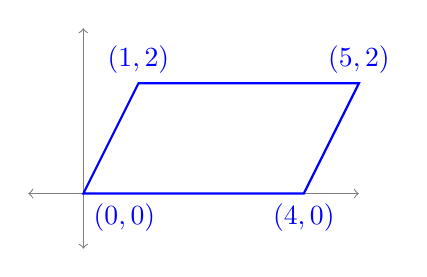
\begin{tikzpicture}[scale=0.7]
\draw[thin,gray,<->] (-1,0)-- (5,0);
\draw[thin,gray,<->] (0,-1)-- (0,3);
\draw[thick,blue] (0,0) node[below right] {$(0,0)$} -- (4,0)node [below] {$(4,0)$} -- (5,2) node[above] {$(5,2)$} -- (1,2) node[above]{$(1,2)$} -- cycle;
\end{tikzpicture}
\end{multicols}

%A
\item Find the area of the parallelogram with vertices $(0,0)$, $(12,5)$, $(12,8)$, and $(0,3)$.
\begin{multicols}{2}
\begin{readinessAssuranceTestChoices}
\item $36$ %Correct
\item $54$
\item $72$
\item $96$
\end{readinessAssuranceTestChoices}


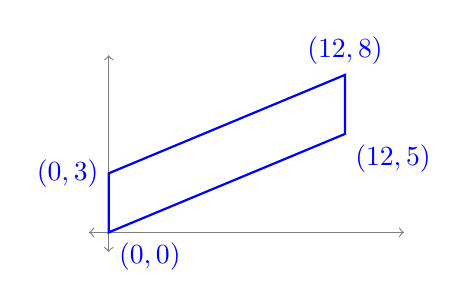
\begin{tikzpicture}[scale=0.25]
\draw[thin,gray,<->] (-1,0)-- (15,0);
\draw[thin,gray,<->] (0,-1)-- (0,9);
\draw[thick,blue] (0,0) node[below right] {$(0,0)$} -- (12,5)node [below right] {$(12,5)$} -- (12,8) node[above] {$(12,8)$} -- (0,3) node[left]{$(0,3)$} -- cycle;
\end{tikzpicture}
\end{multicols}

%D
\item The parallelogram ABCD has area $6$.  If AE is $50\%$ longer than AB, what is the area of the parallelogram AEFD?
\begin{multicols}{2}
\begin{readinessAssuranceTestChoices}
\item $18$
\item $15$
\item $12$
\item $9$  %Correct
\end{readinessAssuranceTestChoices}

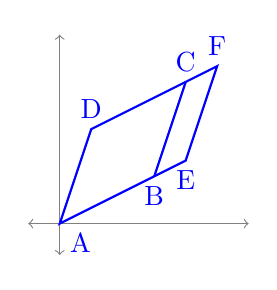
\begin{tikzpicture}[scale=0.4]
\draw[thin,gray,<->] (-1,0)-- (6,0);
\draw[thin,gray,<->] (0,-1)-- (0,6);
\draw[thick,blue] (0,0) node[below right] {A} --(4,2) node[below] {E} -- (5,5) node[above]{F} -- (1,3)node[above] {D} -- cycle;
\draw[thick,blue] (3,1.5) node[below] {B} -- (4,4.5) node [above] {C};
\end{tikzpicture}
\end{multicols}

%C
\item The parallelogram ABCD has area $6$.  If AD is twice as long as AF, what is the area of the parallelogram ABEF?
\begin{multicols}{2}
\begin{readinessAssuranceTestChoices}
\item $1$
\item $2$
\item $3$ %Correct
\item $4$
\end{readinessAssuranceTestChoices}

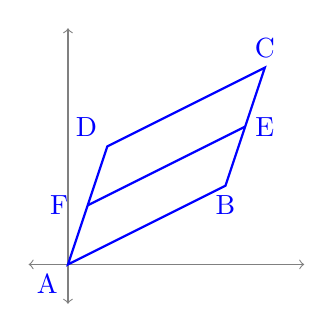
\begin{tikzpicture}[scale=0.5]
\draw[thin,gray,<->] (-1,0)-- (6,0);
\draw[thin,gray,<->] (0,-1)-- (0,6);
\draw[thick,blue] (0,0) node[below left] {A} --(4,2) node[below] {B} -- (5,5) node[above]{C} -- (1,3)node[above left] {D} -- cycle;
\draw[thick,blue] (0.5,1.5) node[left] {F\ \ } -- (4.5,3.5) node [right] {E};
\end{tikzpicture}
\end{multicols}

%A
\item Let $T: \IR^2 \rightarrow \IR$ be a linear transformation.  Which of the following is equal to $2T\left(\begin{bmatrix} a+b \\ a+b \end{bmatrix}\right)$?
\begin{multicols}{2}
\begin{readinessAssuranceTestChoices}
\item $T\left(\begin{bmatrix} a \\ a \end{bmatrix}\right)+T\left(\begin{bmatrix}a \\ b \end{bmatrix} \right)+T\left(\begin{bmatrix}b \\ a \end{bmatrix}\right)+T\left(\begin{bmatrix}b \\ b \end{bmatrix} \right)$ %Correct
\item $T\left(\begin{bmatrix}a \\ b \end{bmatrix} \right)+T\left(\begin{bmatrix}b \\ a \end{bmatrix} \right)$
\item $T\left(\begin{bmatrix}a \\ b \end{bmatrix} \right)$
\item $2T\left(\begin{bmatrix}a \\ b \end{bmatrix} \right)$
\end{readinessAssuranceTestChoices}
\end{multicols}

%D
\item Let $T: \IR^n \rightarrow \IR^n$ be a linear transformation with standard matrix $A$.  Which of the following is equivalent to the statement ``$A$ is an invertible matrix''?
\begin{readinessAssuranceTestChoices}
\item $A$ is a square matrix
\item The matrix equation $AX=B$ has no solution for some $n\times 1$
      matrix $B$.
\item $\RREF(A)$ has a column without a pivot
\item $T$ is both injective and surjective %Correct
\end{readinessAssuranceTestChoices}

%B
\item What is the matrix corresponding to the linear transformation $T: \IR^3 \rightarrow \IR^3$ given by $$T\left( \begin{bmatrix} x \\ y \\ z \end{bmatrix}\right) = \begin{bmatrix} 3x+2y-z \\ y+z \\x+7z \end{bmatrix}?$$
\begin{multicols}{4}
\begin{readinessAssuranceTestChoices}
\item $\begin{bmatrix} 3 & 0 & 1 \\ 2 & 1 & 0 \\ -1 & 1 & 7 \end{bmatrix}$
\item $\begin{bmatrix} 3 & 2 & -1 \\ 0 & 1 & 1 \\ 1 & 0 & 7  \end{bmatrix}$ %Correct
\item $\begin{bmatrix} 3 & 2 & -1 \\ 1 & 1 & 0 \\ 1 & 7 & 0 \end{bmatrix}$
\item $\begin{bmatrix}  3 & 1 & 1 \\ 2 & 1 & 7 \\ -1 & 0 & 0 \end{bmatrix}$
\end{readinessAssuranceTestChoices}
\end{multicols}

%B
\item How many distinct real roots does the polynomial $x^4+3x^3+x^2-3x-2$ have?
(Hint: all the roots are rational.)
\begin{multicols}{4}
\begin{readinessAssuranceTestChoices}
\item $4$
\item $3$ %Correct
\item $2$
\item $1$
\end{readinessAssuranceTestChoices}
\end{multicols}


%A
\item Which of the following is a root of the polynomial $x^2-4x+13$?
\begin{multicols}{4}
\begin{readinessAssuranceTestChoices}
\item $2-3i$ %Correct
\item $3+4i$
\item $4-5i$
\item $5+6i$
\end{readinessAssuranceTestChoices}
\end{multicols}

%A
\item Which of the following conditions imply that the quadratic polynomial $ax^2+bx+c$ has no real roots?
\begin{multicols}{2}
\begin{readinessAssuranceTestChoices}
\item $b^2-4ac<0$ %Correct
\item $a^2+4bc<0$
\item $ac-4b^2<0$
\item $ab+4c^2<0$
\end{readinessAssuranceTestChoices}
\end{multicols}

\end{readinessAssuranceTest}
